% 官方CQ题面逐题译录; 图以自包含TikZ路径重绘.
\originalchapter{官方理解题与解答}\label{ch:official-comprehension}
本章题面译自MIT OpenCourseWare, Paul Seidel的18.900 Geometry and Topology in the Plane, Spring 2023所选第4、29、30、31、33、40讲的Comprehension Questions. 保留官方题号, 共22题. 下列解答均为中文编者补充, 不是MIT官方答案. 前文的编者习题与这些官方题分属不同来源.

第40讲的材料由OCW公开, 但官方课程说明将它列为Spring 2023实际教学中省略的讲次; 本章将其作为公开补充材料收录. 涉及Betti数时采用实数系数. 除第40讲说明的平移曲面记账外, 复形不允许两条不同边具有相同端点.

\originalsection{第4讲: 绕数}
\begin{exercise}\label{cq:4.1}
\textbf{官方题4.1.} 图中的黑点在内部还是外部? 这是一条多边形闭路, 无须检查这一点.
\begin{center}
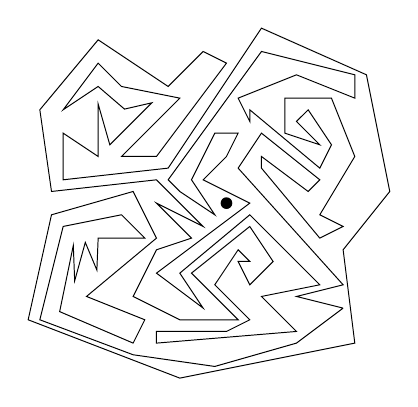
\begin{tikzpicture}[x=1cm,y=1cm,line width=.35pt]
\draw (4.0000,0.8889) --(3.4074,1.0370) --(4.0000,1.1852) --(2.6667,2.6667) --(2.9630,3.1111) --(3.7037,2.5185) --(3.5556,2.3704) --(2.9630,2.8148) --(2.9630,2.6667) --(3.7037,1.7778) --(4.0000,1.9259) --(3.7037,2.0741) --(4.1481,2.8148) --(3.8519,3.5556) --(3.2593,3.5556) --(3.2593,3.1111) --(3.7037,2.9630) --(3.5556,3.1111) --(3.4074,3.2593) --(3.5556,3.4074) --(3.8519,2.9630) --(3.7037,2.6667) --(2.8148,3.4074) --(2.8148,3.2593) --(2.6667,3.5556) --(3.4074,3.8519) --(4.1481,3.5556) --(4.1481,3.8519) --(2.9630,4.1481) --(1.7778,2.5185) --(1.9259,2.3704) --(2.3704,2.0741) --(2.0741,2.5185) --(2.3704,3.1111) --(2.6667,3.1111) --(2.5185,2.8148) --(2.2222,2.5185) --(2.8148,2.2222) --(1.6296,1.3333) --(2.2222,0.8889) --(1.9259,1.3333) --(2.8148,2.0741) --(3.7037,1.1852) --(2.9630,1.0370) --(3.4074,0.5926) --(1.6296,0.4444) --(1.6296,0.5926) --(2.5185,0.5926) --(2.8148,0.7407) --(2.3704,1.1852) --(2.6667,1.6296) --(2.8148,1.4815) --(2.6667,1.4815) --(2.8148,1.1852) --(3.1111,1.4815) --(2.8148,1.9259) --(2.0741,1.3333) --(2.6667,0.7407) --(1.9259,0.7407) --(1.3333,1.0370) --(1.6296,1.6296) --(2.0741,1.7778) --(1.6296,2.2222) --(2.2222,1.9259) --(1.6296,2.5185) --(0.2963,2.3704) --(0.1481,3.4074) --(0.8889,4.2963) --(1.7778,3.7037) --(2.2222,4.1481) --(2.5185,4.0000) --(1.6296,2.8148) --(1.1852,2.8148) --(1.9259,3.5556) --(1.1852,3.7037) --(0.8889,4.0000) --(0.4444,3.4074) --(0.8889,3.7037) --(1.2237,3.4163) --(1.5704,3.4963) --(1.0370,2.9630) --(0.8889,3.4815) --(0.8889,2.8148) --(0.4444,3.1111) --(0.4444,2.5185) --(1.7778,2.6667) --(2.9630,4.4444) --(4.2963,3.8519) --(4.5926,2.3704) --(4.0000,1.6296) --(4.1481,0.4444) --(1.9259,-0.0000) --(0.0000,0.7407) --(0.2963,2.0741) --(1.3333,2.3704) --(1.6296,1.7778) --(0.7407,1.0370) --(1.4815,0.7407) --(1.3333,0.4444) --(0.4000,0.8444) --(0.5733,1.6844) --(0.5907,1.2351) --(0.7257,1.7235) --(0.8726,1.3723) --(0.8889,1.7778) --(1.4815,1.7778) --(1.1852,2.0741) --(0.4444,1.9259) --(0.1481,0.7407) --(1.3333,0.2963) --(2.3704,0.1481) --(3.4074,0.4444) --(4.0000,0.8889);
\fill (2.5185,2.2222) circle (0.0741);
\end{tikzpicture}
\end{center}
\end{exercise}
\begin{solution}
在内部. 从黑点向右略向上作射线, 例如取斜率$0.01$, 与边界相交5次且避开顶点. 每穿过一次边界就在内部与外部之间切换; 射线终端在外部, 交点数为奇数, 所以起点在内部. 这正是第4讲公式(4.10)的奇偶判别.
\end{solution}

\begin{exercise}\label{cq:4.2}
\textbf{官方题4.2.} 计算按箭头方向行进时围绕黑点的绕数.
\begin{center}
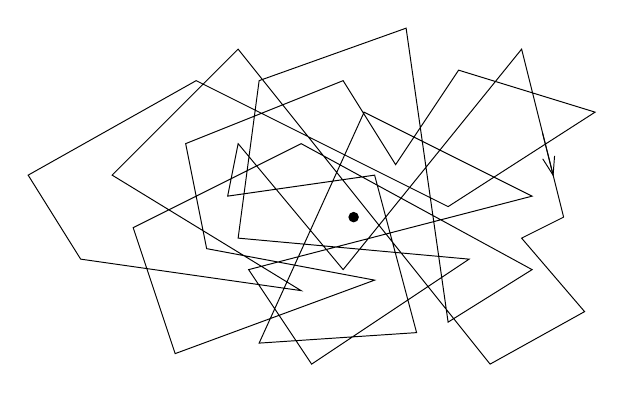
\begin{tikzpicture}[x=1cm,y=1cm,line width=.35pt]
\fill (4.1333,1.8667) circle (0.0667);
\draw (6.8000,1.8667) --(6.2667,4.0000) --(4.0000,1.2000) --(2.6667,2.8000) --(2.5333,2.1333) --(4.4000,2.4000) --(4.9333,0.4000) --(2.9333,0.2667) --(4.2667,3.2000) --(6.4000,2.1333) --(2.8000,1.2000) --(3.6000,0.0000) --(5.6000,1.3333) --(2.6667,1.6000) --(2.9333,3.6000) --(4.8000,4.2667) --(5.3333,0.5333) --(6.4000,1.2000) --(3.4667,2.8000) --(1.3333,1.7333) --(1.8667,0.1333) --(4.4000,1.0667) --(2.2667,1.4667) --(2.0000,2.8000) --(4.0000,3.6000) --(4.6667,2.5333) --(5.4667,3.7333) --(7.2000,3.2000) --(5.3333,2.0000) --(2.1333,3.6000) --(0.0000,2.4000) --(0.6667,1.3333) --(3.4667,0.9333) --(1.0667,2.4000) --(2.6667,4.0000) --(5.8667,0.0000) --(7.0667,0.6667) --(6.2667,1.6000) --(6.8000,1.8667);
\draw (6.5333,2.9333) --(6.6667,2.4000);
\draw (6.6855,2.6452) --(6.6667,2.4000) --(6.5347,2.6075);
\end{tikzpicture}
\end{center}
\end{exercise}
\begin{solution}
绕数为$3$. 从黑点向右略向上作射线, 避开顶点和交叉点. 从近到远, 七次穿越按第4讲公式(4.9)的约定依次贡献$+1,+1,+1,+1,-1,+1,-1$, 总和为$3$. 这里正号表示曲线在交点沿射线的左法向穿过. 必须沿题图箭头取向; 反向绕行会得到$-3$.
\end{solution}

\begin{exercise}\label{cq:4.3}
\textbf{官方题4.3.} 仿照第4讲例4.7, 对下图逐步使用消除自交点的方法, 并记录每一步绕数怎样改变.
\begin{center}
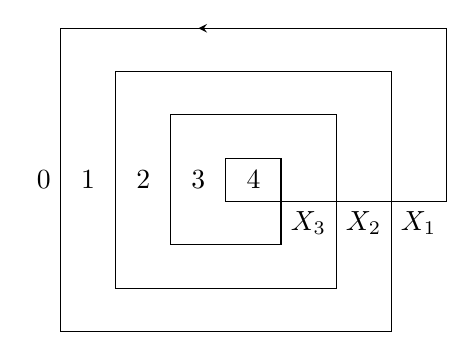
\begin{tikzpicture}[x=.7cm,y=.55cm,line width=.4pt,>=stealth]
\draw (0.000,0.000) -- (0.000,-7.000) -- (6.000,-7.000) -- (6.000,-1.000) -- (1.000,-1.000) -- (1.000,-6.000) -- (5.000,-6.000) -- (5.000,-2.000) -- (2.000,-2.000) -- (2.000,-5.000) -- (4.000,-5.000) -- (4.000,-3.000) -- (3.000,-3.000) -- (3.000,-4.000) -- (7.000,-4.000) -- (7.000,0.000) -- cycle;
\draw[->] (4,0)--(2.5,0);
\foreach \i in {1,...,4}{\node at (\i-.5,-3.5) {$\i$};}
\node[left] at (0,-3.5) {$0$};
\foreach \x/\i in {6/1,5/2,4/3}{\node[below right] at (\x,-4) {$X_{\i}$};}
\end{tikzpicture}
\end{center}
\end{exercise}
\begin{solution}
图中外部绕数为$0$, 四个有界区域的初始绕数依次为$1,2,3,4$. 记它们为$R_1,R_2,R_3,R_4$, 将三个交叉点从外到内标作$X_1,X_2,X_3$. 图中的这些数字及$X_i$为编者增加的标记.

依次处理$X_1,X_2,X_3$. 每次将交叉处分成的两段闭路中较内的一段反向, 再在一个不含其他交点的小圆盘内连接邻近的两端, 使结果仍为一条闭路. 下图给出依次得到的闭路; 顶部箭头保持原方向.
\begin{center}
\begin{tikzpicture}[x=.4cm,y=.34cm,line width=.4pt,>=stealth]
\begin{scope}[xshift=0.0cm]
\draw (0.000,0.000) -- (0.000,-7.000) -- (6.000,-7.000) -- (6.000,-4.150) -- (5.850,-4.000) -- (3.000,-4.000) -- (3.000,-3.000) -- (4.000,-3.000) -- (4.000,-5.000) -- (2.000,-5.000) -- (2.000,-2.000) -- (5.000,-2.000) -- (5.000,-6.000) -- (1.000,-6.000) -- (1.000,-1.000) -- (6.000,-1.000) -- (6.000,-3.850) -- (6.150,-4.000) -- (7.000,-4.000) -- (7.000,0.000) -- cycle;
\draw[->] (4,0)--(2.5,0);
\node at (3.5,-8.1) {第1步};
\end{scope}
\begin{scope}[xshift=3.3cm]
\draw (0.000,0.000) -- (0.000,-7.000) -- (6.000,-7.000) -- (6.000,-4.150) -- (5.850,-4.000) -- (5.150,-4.000) -- (5.000,-3.850) -- (5.000,-2.000) -- (2.000,-2.000) -- (2.000,-5.000) -- (4.000,-5.000) -- (4.000,-3.000) -- (3.000,-3.000) -- (3.000,-4.000) -- (4.850,-4.000) -- (5.000,-4.150) -- (5.000,-6.000) -- (1.000,-6.000) -- (1.000,-1.000) -- (6.000,-1.000) -- (6.000,-3.850) -- (6.150,-4.000) -- (7.000,-4.000) -- (7.000,0.000) -- cycle;
\draw[->] (4,0)--(2.5,0);
\node at (3.5,-8.1) {第2步};
\end{scope}
\begin{scope}[xshift=6.6cm]
\draw (0.000,0.000) -- (0.000,-7.000) -- (6.000,-7.000) -- (6.000,-4.150) -- (5.850,-4.000) -- (5.150,-4.000) -- (5.000,-3.850) -- (5.000,-2.000) -- (2.000,-2.000) -- (2.000,-5.000) -- (4.000,-5.000) -- (4.000,-4.150) -- (3.850,-4.000) -- (3.000,-4.000) -- (3.000,-3.000) -- (4.000,-3.000) -- (4.000,-3.850) -- (4.150,-4.000) -- (4.850,-4.000) -- (5.000,-4.150) -- (5.000,-6.000) -- (1.000,-6.000) -- (1.000,-1.000) -- (6.000,-1.000) -- (6.000,-3.850) -- (6.150,-4.000) -- (7.000,-4.000) -- (7.000,0.000) -- cycle;
\draw[->] (4,0)--(2.5,0);
\node at (3.5,-8.1) {第3步};
\end{scope}
\end{tikzpicture}
\end{center}
在远离三个小圆盘的原区域内各固定一点, 绕数的变化如下. 表中$R_0$表示原外部; 同值区域有时会因消除交点而合并.
\begin{center}
\begin{tabular}{c|rrrrr}
 & $R_0$ & $R_1$ & $R_2$ & $R_3$ & $R_4$ \\\hline
初始 & $0$ & $1$ & $2$ & $3$ & $4$ \\
消除$X_1$后 & $0$ & $1$ & $0$ & $-1$ & $-2$ \\
再消除$X_2$后 & $0$ & $1$ & $0$ & $1$ & $2$ \\
再消除$X_3$后 & $0$ & $1$ & $0$ & $1$ & $0$
\end{tabular}
\end{center}
为核对这些数, 令$L_1,L_2,L_3,L_4$是把原交叉处拆开后得到的四条逆时针嵌套简单闭路, 从外到内编号. 初始绕数是四个$\operatorname{wind}(L_j,q)$之和; 三次反向操作后的系数依次为$(1,-1,-1,-1)$、$(1,-1,1,1)$、$(1,-1,1,-1)$. 在$R_j$内恰有前$j$条闭路的绕数等于$1$, 求部分和即得全表. 局部改接不影响圆盘外固定点的绕数, 因为连续变形过程中没有经过这些点.
\end{solution}

\begin{exercise}\label{cq:4.4}
\textbf{官方题4.4.} 一条多边形闭路只有简单自交点, 且恰有4个这样的自交点. 它能有的最大绕数是多少? 解释, 并画出达到最大绕数的例子.
\end{exercise}
\begin{solution}
最大为$5$. 一般地, 在自交点把有向闭路拆成两条有向闭路时, 原绕数等于两条闭路绕数之和. 持续拆开各闭路自身的交点, 最后至多得到$N+1$条简单闭路, 因为每次拆开增加一条闭路, 并消去至少一个原交点. 每条简单闭路在给定点的绕数属于$\{-1,0,1\}$, 所以$|\operatorname{wind}|\le N+1$. 两条拆开后的闭路之间即使还有相交, 也不影响各自为简单闭路的判断及绕数的可加性.

下面的五层方形螺旋恰有4个简单自交点. 黑点$q$位于五个逆时针圈共同包围的区域, 向右射线的五次穿越都贡献$+1$, 因而绕数为$5$.
\begin{center}
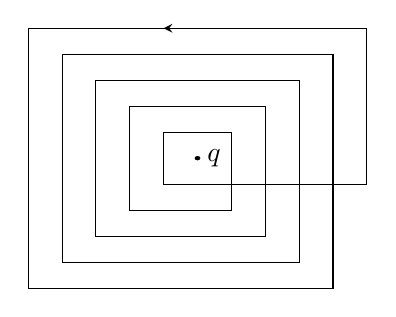
\begin{tikzpicture}[x=.43cm,y=.33cm,line width=.4pt,>=stealth]
\draw (0.000,0.000) -- (0.000,-10.000) -- (9.000,-10.000) -- (9.000,-1.000) -- (1.000,-1.000) -- (1.000,-9.000) -- (8.000,-9.000) -- (8.000,-2.000) -- (2.000,-2.000) -- (2.000,-8.000) -- (7.000,-8.000) -- (7.000,-3.000) -- (3.000,-3.000) -- (3.000,-7.000) -- (6.000,-7.000) -- (6.000,-4.000) -- (4.000,-4.000) -- (4.000,-6.000) -- (10.000,-6.000) -- (10.000,0.000) -- cycle;
\draw[->] (6,0)--(4,0);
\fill (5,-5) circle (.085);
\node[right] at (5,-5) {$q$};
\end{tikzpicture}
\end{center}
\end{solution}

\originalsection{第29讲: 边界矩阵}
本组题的官方说明要求只用截至第29讲已介绍的材料; 不能预先使用下一讲关于平面复形Betti数的结论. 本节解答遵守这一限制.

\begin{exercise}\label{cq:29.1}
\textbf{官方题29.1.} 哪些图是平面复形, 哪些不是? 与讲义相同, 属于复形的顶点均画成粗黑点, 属于复形的三角形均涂灰. 四幅图从左到右依次编号为(a)--(d).
\begin{center}
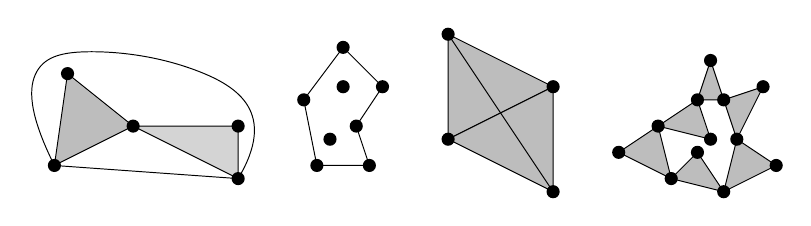
\begin{tikzpicture}[x=1cm,y=1cm,line width=.35pt]
\draw[fill=black!26] (1.3333,0.9167) --(0.3333,0.4167) --(0.5000,1.5833) --(1.3333,0.9167);
\draw[fill=black!26] (5.3333,0.7500) --(5.3333,2.0833) --(6.6667,1.4167) --(5.3333,0.7500);
\draw[fill=black!26] (6.6667,0.0833) --(5.3333,0.7500) --(6.6667,1.4167) --(6.6667,0.0833);
\draw[fill=black!17] (2.6667,0.2500) --(1.3333,0.9167) --(2.6667,0.9167) --(2.6667,0.2500);
\fill (1.3333,0.9167) circle (0.0833);
\fill (2.6667,0.2500) circle (0.0833);
\fill (2.6667,0.9167) circle (0.0833);
\fill (5.3333,2.0833) circle (0.0833);
\fill (6.6667,1.4167) circle (0.0833);
\fill (5.3333,0.7500) circle (0.0833);
\fill (6.6667,0.0833) circle (0.0833);
\draw (5.3333,2.0833) --(6.6667,0.0833);
\draw[fill=black!26] (8.1667,0.2500) --(7.5000,0.5833) --(8.0000,0.9167) --(8.1667,0.2500);
\draw[fill=black!26] (8.6667,0.7500) --(8.0000,0.9167) --(8.5000,1.2500) --(8.6667,0.7500);
\draw[fill=black!26] (8.8333,0.0833) --(8.1667,0.2500) --(8.5000,0.5833) --(8.8333,0.0833);
\draw[fill=black!26] (8.8333,0.0833) --(9.0000,0.7500) --(9.5000,0.4167) --(8.8333,0.0833);
\draw[fill=black!26] (9.0000,0.7500) --(9.3333,1.4167) --(8.8333,1.2500) --(9.0000,0.7500);
\draw[fill=black!26] (8.8333,1.2500) --(8.5000,1.2500) --(8.6667,1.7500) --(8.8333,1.2500);
\fill (7.5000,0.5833) circle (0.0833);
\fill (8.0000,0.9167) circle (0.0833);
\fill (8.1667,0.2500) circle (0.0833);
\fill (8.5000,0.5833) circle (0.0833);
\fill (8.6667,0.7500) circle (0.0833);
\fill (8.5000,1.2500) circle (0.0833);
\fill (8.6667,1.7500) circle (0.0833);
\fill (8.8333,1.2500) circle (0.0833);
\fill (9.3333,1.4167) circle (0.0833);
\fill (9.0000,0.7500) circle (0.0833);
\fill (9.5000,0.4167) circle (0.0833);
\fill (8.8333,0.0833) circle (0.0833);
\draw (4.5000,1.4167) --(4.0000,1.9167) --(3.5000,1.2500) --(3.6667,0.4167) --(4.3333,0.4167) --(4.1667,0.9167) --(4.5000,1.4167);
\fill (4.0000,1.9167) circle (0.0833);
\fill (3.5000,1.2500) circle (0.0833);
\fill (4.0000,1.4167) circle (0.0833);
\fill (3.8333,0.7500) circle (0.0833);
\fill (3.6667,0.4167) circle (0.0833);
\fill (4.3333,0.4167) circle (0.0833);
\fill (4.1667,0.9167) circle (0.0833);
\fill (4.5000,1.4167) circle (0.0833);
\fill (0.5000,1.5833) circle (0.0833);
\fill (0.3333,0.4167) circle (0.0833);
\draw (2.6667,0.2500) .. controls (3.1667,1.0833) and (2.6667,1.4167) ..(2.1667,1.6111) .. controls (1.6667,1.8055) and (1.1667,1.8611) ..(0.8055,1.8611) .. controls (0.4445,1.8611) and (0.2222,1.8055) ..(0.1111,1.6111) .. controls (0.0000,1.4167) and (0.0000,1.0833) ..(0.3333,0.4167);
\draw (0.3333,0.4167) --(2.6667,0.2500);
\end{tikzpicture}
\end{center}
\end{exercise}
\begin{solution}
(b)、(d)是平面复形, (a)、(c)不是. (a)中的外侧曲边不是线段, 违反平面复形的直边要求; 内部还画出了相同两端点之间的直边. (c)中的两条对角线在没有黑点处相交, 另画的对角线穿过灰三角形的内部. (b)允许有孤立顶点及未填充的多边形区域, 所以内部的黑点无妨. (d)中各三角形只共用整条边或顶点, 且每个三角形的边、每条边的端点都在图中, 满足全部条件.
\end{solution}

\begin{exercise}\label{cq:29.2}
\textbf{官方题29.2.} 给定下列边界矩阵, 画出复形:
\[
D_1=\begin{pmatrix}
-1&-1&-1&-1&0&0&0\\
1&0&0&0&-1&-1&0\\
0&1&0&0&1&0&-1\\
0&0&1&0&0&1&1\\
0&0&0&1&0&0&0
\end{pmatrix},\qquad
D_2=\begin{pmatrix}
1&0&0\\-1&1&0\\0&-1&0\\0&0&0\\1&0&1\\0&0&-1\\0&1&1
\end{pmatrix}.
\]
\end{exercise}
\begin{solution}
$D_1$的列依次给出边$12,13,14,15,23,24,34$. 按这个边顺序读取$D_2$的三列, 得面$123,134,234$. 取$3$为三角形$124$的内部顶点, 将大三角形分成三面, 再从$1$接一条伸向外部顶点$5$的边, 即得所求图.
\begin{center}
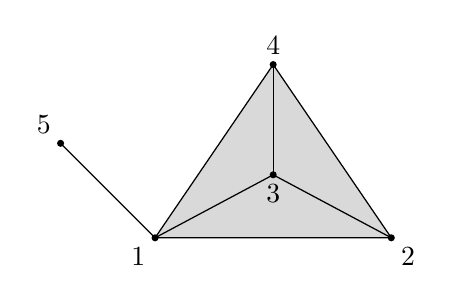
\begin{tikzpicture}[x=1cm,y=1cm,line width=.45pt]
\coordinate (v1) at (0,0); \coordinate (v2) at (3,0);
\coordinate (v3) at (1.5,.8); \coordinate (v4) at (1.5,2.2);
\coordinate (v5) at (-1.2,1.2);
\fill[black!15] (v1)--(v2)--(v4)--cycle;
\draw (v1)--(v2)--(v4)--cycle;
\draw (v1)--(v3)--(v2); \draw (v3)--(v4); \draw (v1)--(v5);
\foreach \i in {1,2,3,4,5}{\fill (v\i) circle (.045);}
\node[below left] at (v1) {$1$}; \node[below right] at (v2) {$2$};
\node[below] at (v3) {$3$}; \node[above] at (v4) {$4$}; \node[above left] at (v5) {$5$};
\end{tikzpicture}
\end{center}
\end{solution}

\begin{exercise}\label{cq:29.3}
\textbf{官方题29.3.} 哪些整数能成为平面复形的欧拉示性数? 对能出现的每个值给出例子, 对不能出现的值给出解释.
\end{exercise}
\begin{solution}
每个整数都能出现. 对$m\ge1$, 取$m$个孤立顶点, 得$\chi=m$. 对$m\le0$, 令$r=1-m$, 在互不重叠的角形扇区内画$r$个三角形的边界, 所有边界仅共用一个顶点, 不填面. 此时$V=1+2r$, $E=3r$, $F=0$, 所以$\chi=1-r=m$. 每条边都是线段, 不同三角形只在公共顶点相交, 确实是平面复形. 这些计数不需要下一讲的孔洞公式.
\end{solution}

\begin{exercise}\label{cq:29.4}
\textbf{官方题29.4.} 计算一个三角形的Betti数. 这里三角形包含填充的内部, 即$n_0=3,n_1=3,n_2=1$.
\end{exercise}
\begin{solution}
三条边的边界生成二维空间$\{(x_1,x_2,x_3):x_1+x_2+x_3=0\}$, 所以$\operatorname{rank}D_1=2$. 唯一面的边界非零, 所以$\operatorname{rank}D_2=1$. 代入定理\ref{thm:euler-poincare}, 得$(b_0,b_1,b_2)=(1,0,0)$.
\end{solution}

\originalsection{第30讲: Betti数}
\begin{exercise}\label{cq:30.1}
\textbf{官方题30.1.} 假设下图的灰色部分已分解成三角形, 使整体成为复形. 计算它的Betti数.
\begin{center}
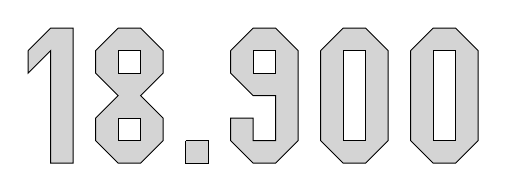
\begin{tikzpicture}[x=1cm,y=1cm,line width=.35pt]
\draw[fill=black!17] (0.0000,1.4286) --(0.2857,1.7143) --(0.5714,1.7143) --(0.5714,0.0000) --(0.2857,0.0000) --(0.2857,1.4286) --(0.0000,1.1429) --(0.0000,1.4286);
\draw[fill=black!17] (1.1429,1.7143) --(0.8571,1.4286) --(0.8571,1.1429) --(1.1429,0.8571) --(0.8571,0.5714) --(0.8571,0.2857) --(1.1429,0.0000) --(1.4286,0.0000) --(1.7143,0.2857) --(1.7143,0.5714) --(1.4286,0.8571) --(1.7143,1.1429) --(1.7143,1.4286) --(1.4286,1.7143) --(1.1429,1.7143);
\draw[fill=black!0] (1.1429,1.1429) rectangle (1.4286,1.4286);
\draw[fill=black!0] (1.1429,0.2857) rectangle (1.4286,0.5714);
\draw[fill=black!17] (2.0000,0.2857) --(2.0000,0.0000) --(2.2857,0.0000) --(2.2857,0.2857) --(2.0000,0.2857);
\draw[fill=black!17] (2.5714,1.4286) --(2.8571,1.7143) --(3.1429,1.7143) --(3.4286,1.4286) --(3.4286,0.2857) --(3.1429,0.0000) --(2.8571,0.0000) --(2.5714,0.2857) --(2.5714,0.5714) --(2.8571,0.5714) --(2.8571,0.2857) --(3.1429,0.2857) --(3.1429,0.8571) --(2.8571,0.8571) --(2.5714,1.1429) --(2.5714,1.4286);
\draw[fill=black!0] (2.8571,1.1429) rectangle (3.1429,1.4286);
\draw[fill=black!17] (3.7143,1.4286) --(4.0000,1.7143) --(4.2857,1.7143) --(4.5714,1.4286) --(4.5714,0.2857) --(4.2857,0.0000) --(4.0000,0.0000) --(3.7143,0.2857) --(3.7143,1.4286);
\draw[fill=black!0] (4.0000,0.2857) rectangle (4.2857,1.4286);
\draw (2.0000,0.2857) --(2.0000,0.2857);
\draw[fill=black!17] (4.8571,1.4286) --(5.1429,1.7143) --(5.4286,1.7143) --(5.7143,1.4286) --(5.7143,0.2857) --(5.4286,0.0000) --(5.1429,0.0000) --(4.8571,0.2857) --(4.8571,1.4286);
\draw[fill=black!0] (5.1429,0.2857) rectangle (5.4286,1.4286);
\end{tikzpicture}
\end{center}
\end{exercise}
\begin{solution}
$(b_0,b_1,b_2)=(6,5,0)$. 字形$1,8,\text{小数点},9,0,0$是六个分支. $8$有两个孔洞, $9$及两个$0$各有一个, 合计五个; $1$与小数点没有孔洞. 用第30讲定理30.2及推论30.5, 平面复形的$b_2=0$, $b_1$等于有界补集分支数, 就得到这些值. 小数点是填充的小方块, 不能忽略其连通分支.
\end{solution}

\begin{exercise}\label{cq:30.2}
\textbf{官方题30.2.} 画一个满足$b_0=3,b_1=3$的平面复形.
\end{exercise}
\begin{solution}
取三个相互分离、内部不填充的三角形边界:
\begin{center}
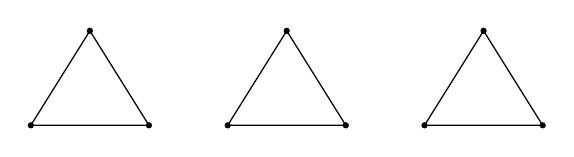
\begin{tikzpicture}[x=1cm,y=1cm,line width=.45pt]
\foreach \x in {0,2.5,5}{
\draw (\x,0)--(\x+1.5,0)--(\x+.75,1.2)--cycle;
\fill (\x,0) circle (.04); \fill (\x+1.5,0) circle (.04); \fill (\x+.75,1.2) circle (.04);}
\end{tikzpicture}
\end{center}
每个分支有$V=E=3$, $F=0$, $\operatorname{rank}D_1=2$, 所以每个的Betti数为$(1,1,0)$. 三个分支的矩阵互不混合, 总Betti数为$(3,3,0)$.
\end{solution}

\begin{exercise}\label{cq:30.3}
\textbf{官方题30.3.} 两个抽象复形的不交并, 是将它们各自的顶点、边和三角形直接合在一起, 并将两套对象视为不同对象. 若$K=K_1\sqcup K_2$, 它们的Betti数有何关系? 为什么?
\end{exercise}
\begin{solution}
对$i=0,1,2$, 有$b_i(K)=b_i(K_1)+b_i(K_2)$. 先列$K_1$的基, 再列$K_2$的基, 两个边界矩阵就都成为对应矩阵的块对角和. 块对角矩阵的秩等于两块的秩之和, 各维单形数也相加; 将这些等式代入定理\ref{thm:euler-poincare}的三个公式即得结论. 等价地, 同调向量空间本身也是两个同调空间的直和.
\end{solution}

\begin{exercise}\label{cq:30.4}
\textbf{官方题30.4.} 将M\"obius带构造成一个抽象复形, 并计算它的Betti数. 注意按本课程的定义, 不允许不同边具有相同的端点. 允许用计算机辅助计算矩阵的秩.
\end{exercise}
\begin{solution}
将一个长方形分成三个小方格, 每格从左上角连到右下角, 再将左右两边反向粘合. 六个不同顶点记作$a_0,a_1,a_2,b_0,b_1,b_2$, 并约定$a_3=b_0,b_3=a_0$. 六个面的顶点集为
\[
\{a_i,b_i,b_{i+1}\},\quad \{a_i,a_{i+1},b_{i+1}\},\qquad i=0,1,2.
\]
边取这些面的全部二元子集. 图中相同字母表示同一顶点, 两侧箭头表示实际粘合方向.
\begin{center}
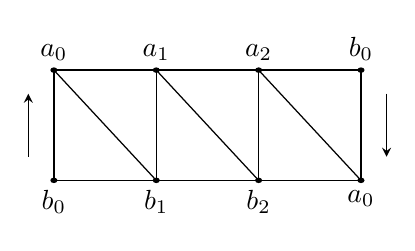
\begin{tikzpicture}[x=1.3cm,y=1cm,line width=.45pt,>=stealth]
\draw (0,0) rectangle (3,1.4);
\foreach \i in {0,1,2}{\draw (\i,1.4)--(\i+1,0);}
\foreach \i in {1,2}{\draw (\i,0)--(\i,1.4);}
\foreach \i/\a/\b in {0/a_0/b_0,1/a_1/b_1,2/a_2/b_2,3/b_0/a_0}{
\fill (\i,1.4) circle (.035); \fill (\i,0) circle (.035);
\node[above] at (\i,1.4) {$\a$}; \node[below] at (\i,0) {$\b$};}
\draw[->] (-.25,.3)--(-.25,1.1); \draw[->] (3.25,1.1)--(3.25,.3);
\end{tikzpicture}
\end{center}
边恰有三条$a_ib_i$、三条$a_ib_{i+1}$及六条边界边$a_ia_{i+1},b_ib_{i+1}$, 共12条; 代入端点约定检查可知没有重复的无序端点对. 面的顶点集也两两不同. 因而这确为抽象复形, 几何实现正是上述反向粘合得到的M\"obius带.

它连通, 故$\operatorname{rank}D_1=V-1=5$. 每个三角形各有一条只属于该面的边界边, 所以$D_2t=0$时沿这些边逐一读出该面系数为零; 六列独立, $\operatorname{rank}D_2=6$. 因此$V=6,E=12,F=6$给出$(b_0,b_1,b_2)=(1,1,0)$. 这也与$\chi=0$一致.
\end{solution}

\begin{exercise}\label{cq:30.5}
\textbf{官方题30.5.} 平面上有$v_1=(0,0),v_2=(1,0),v_3=(0,1),v_4=(1,1)$. 尺度$\sigma=0.7,1.1,1.5$时的Vietoris--Rips复形各是什么?
\end{exercise}
\begin{solution}
四条正方形边长为$1$, 两条对角线长为$\sqrt2$. 按第30讲的定义, 两点距离小于$\sigma$就加边, 三点两两距离小于$\sigma$就填三角形.
\begin{enumerate}[label=(\arabic*)]
\item $\sigma=0.7$: 只有四个孤立顶点, 没有边或面.
\item $\sigma=1.1$: 有边$12,13,24,34$, 即正方形边界, 没有面; 任意三个顶点都包含一对对角点.
\item $\sigma=1.5$: 有全部六条边和四个三角面$123,124,134,234$, 是抽象四面体的边界.
\end{enumerate}
本课程的复形定义只保留到二维, 所以最后一个模型没有三维四面体内部. 若采用通常的全维Vietoris--Rips定义, 最后一项还应包含一个三维单形; 这不是本题采用的约定. 前述三个二维模型的Betti数分别为$(4,0,0)$、$(1,1,0)$、$(1,0,1)$, 最后一项也见\hyperlink{example.14.1}{例题14.1}.
\end{solution}

\originalsection{第31讲: 组合曲面}
\begin{exercise}\label{cq:31.1}
\textbf{官方题31.1.} 将两个四面体在一个顶点粘在一起. 结果是曲面吗? 简短解释.
\begin{center}
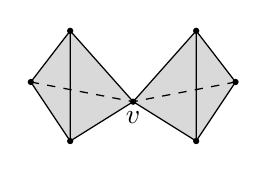
\begin{tikzpicture}[x=1cm,y=1cm,line width=.45pt]
\coordinate (v) at (0,0);
\coordinate (a) at (-.8,.9); \coordinate (b) at (-1.3,.25); \coordinate (c) at (-.8,-.5);
\coordinate (d) at (.8,.9); \coordinate (e) at (1.3,.25); \coordinate (f) at (.8,-.5);
\fill[black!15] (a)--(b)--(c)--(v)--cycle;
\fill[black!15] (d)--(e)--(f)--(v)--cycle;
\draw (a)--(b)--(c)--(v)--(a)--(c); \draw[dashed] (b)--(v);
\draw (d)--(e)--(f)--(v)--(d)--(f); \draw[dashed] (e)--(v);
\foreach \p in {v,a,b,c,d,e,f}{\fill (\p) circle (.04);}
\node[below] at (v) {$v$};
\end{tikzpicture}
\end{center}
\end{exercise}
\begin{solution}
不是. 粘合点$v$的链环是两个互不相交的三角形圆周, 而非一个圆周, 违反第14章的顶点局部条件. 等价地, 其足够小邻域删去$v$后分成两部分, 而圆盘邻域删去中心仍连通. 每条边邻接两面这一条件单独不能保证是曲面.
\end{solution}

\begin{exercise}\label{cq:31.2}
\textbf{官方题31.2.} 明确证明八面体可定向.
\end{exercise}
\begin{solution}
将上下两个顶点记为$N,S$, 赤道四个顶点依次记为$v_0,v_1,v_2,v_3$, 下标模$4$. 给四个上半面的方向$[N,v_i,v_{i+1}]$, 四个下半面的方向$[S,v_{i+1},v_i]$.

在赤道边$v_iv_{i+1}$上, 上面沿$v_i\to v_{i+1}$, 下面沿反方向. 在边$Nv_i$上, 相邻的两个上半面分别沿$N\to v_i$和$v_i\to N$; $Sv_i$同理. 这些是全部边, 故每条共边两侧的诱导方向相反, 所列八个方向组成定向.
\end{solution}

\begin{exercise}\label{cq:31.3}
\textbf{官方题31.3.} 讲义指出曲面的三角形个数必为偶数. 为什么?
\end{exercise}
\begin{solution}
按本讲的闭组合曲面定义, 每个三角形有3条边, 每条边恰邻接2个三角形. 对面边关联计数, 得$3F=2E$, 因而$F$为偶数. 这里不能直接套到有边界曲面, 其边界边只邻接一个三角形.
\end{solution}

\begin{exercise}\label{cq:31.4}
\textbf{官方题31.4.} 是否存在欧拉示性数为$3$的曲面? 允许任意多个连通分支. 若存在, 举例; 若不存在, 解释.
\end{exercise}
\begin{solution}
存在: 取球面与实射影平面的不交并$S^2\sqcup\mathbb RP^2$. 球面的四面体边界模型有$\chi=4-6+4=2$; 射影平面的组合模型有$\chi=1$, 见\hyperlink{example.14.2}{例题14.2}. 两者先采用互不相交的顶点集, 不交并的顶点、边、面数分别相加, 故总欧拉数为$2+1=3$. 该曲面有一个不可定向分支, 与命题\ref{thm:orientable-even}不冲突.
\end{solution}

\begin{exercise}\label{cq:31.5}
\textbf{官方题31.5.} 第6讲的三角形铺砌(6.9)、(6.11)是周期的, 所以各自都能给出一个环面的组合版本. 画出这两个曲面. 注意按本课程的定义, 不允许不同边具有相同端点.
\end{exercise}
\begin{solution}
下面画的是两个足够大的周期平行四边形, 同向箭头所标的两对边分别按平移粘合. 顶点与边界上的中点也依同一平移配对. 图中的黑点是三角剖分顶点; 四个角都记作$v_{00}$, 其余重复的边界顶点按下述周期规则识别.
\begin{center}
\begin{tikzpicture}[x=.75cm,y=.75cm,line width=.35pt,>=stealth]
\draw (0,0)--(0,4);
\draw (0,0)--(4,0);
\draw (1,0)--(1,4);
\draw (0,1)--(4,1);
\draw (2,0)--(2,4);
\draw (0,2)--(4,2);
\draw (3,0)--(3,4);
\draw (0,3)--(4,3);
\draw (4,0)--(4,4);
\draw (0,4)--(4,4);
\draw (0.00000,0.00000)--(1.00000,1.00000);
\draw (1.00000,1.00000)--(0.00000,2.00000);
\draw (0.00000,2.00000)--(1.00000,3.00000);
\draw (1.00000,3.00000)--(0.00000,4.00000);
\draw (2.00000,0.00000)--(1.00000,1.00000);
\draw (1.00000,1.00000)--(2.00000,2.00000);
\draw (2.00000,2.00000)--(1.00000,3.00000);
\draw (1.00000,3.00000)--(2.00000,4.00000);
\draw (2.00000,0.00000)--(3.00000,1.00000);
\draw (3.00000,1.00000)--(2.00000,2.00000);
\draw (2.00000,2.00000)--(3.00000,3.00000);
\draw (3.00000,3.00000)--(2.00000,4.00000);
\draw (4.00000,0.00000)--(3.00000,1.00000);
\draw (3.00000,1.00000)--(4.00000,2.00000);
\draw (4.00000,2.00000)--(3.00000,3.00000);
\draw (3.00000,3.00000)--(4.00000,4.00000);
\fill (0,0) circle (.035);
\fill (0,1) circle (.035);
\fill (0,2) circle (.035);
\fill (0,3) circle (.035);
\fill (0,4) circle (.035);
\fill (1,0) circle (.035);
\fill (1,1) circle (.035);
\fill (1,2) circle (.035);
\fill (1,3) circle (.035);
\fill (1,4) circle (.035);
\fill (2,0) circle (.035);
\fill (2,1) circle (.035);
\fill (2,2) circle (.035);
\fill (2,3) circle (.035);
\fill (2,4) circle (.035);
\fill (3,0) circle (.035);
\fill (3,1) circle (.035);
\fill (3,2) circle (.035);
\fill (3,3) circle (.035);
\fill (3,4) circle (.035);
\fill (4,0) circle (.035);
\fill (4,1) circle (.035);
\fill (4,2) circle (.035);
\fill (4,3) circle (.035);
\fill (4,4) circle (.035);
\draw[->] (1,-.3)--(3,-.3); \draw[->] (1,4.3)--(3,4.3);
\draw[->] (-.3,1)--(-.3,3); \draw[->] (4.3,1)--(4.3,3);
\node at (2,-.85) {(6.9) 的周期商};
\node[below left] at (0,0) {$v_{00}$};
\node[below right] at (4,0) {$v_{00}$};
\node[above left] at (0,4) {$v_{00}$};
\node[above right] at (4,4) {$v_{00}$};
\begin{scope}[xshift=5.3cm]
\draw (0.00000,0.00000)--(1.00000,0.00000);
\draw (1.00000,0.00000)--(0.50000,0.86603);
\draw (0.50000,0.86603)--(0.00000,0.00000);
\draw (0.00000,0.00000)--(0.75000,0.43301);
\draw (0.50000,0.86603)--(1.50000,0.86603);
\draw (1.50000,0.86603)--(1.00000,0.00000);
\draw (1.50000,0.86603)--(0.75000,0.43301);
\draw (1.50000,0.86603)--(1.00000,1.73205);
\draw (1.00000,1.73205)--(0.50000,0.86603);
\draw (1.50000,0.86603)--(0.75000,1.29904);
\draw (1.00000,1.73205)--(2.00000,1.73205);
\draw (2.00000,1.73205)--(1.50000,0.86603);
\draw (1.50000,0.86603)--(1.50000,1.73205);
\draw (2.00000,1.73205)--(1.50000,2.59808);
\draw (1.50000,2.59808)--(1.00000,1.73205);
\draw (1.50000,2.59808)--(1.50000,1.73205);
\draw (1.50000,2.59808)--(2.50000,2.59808);
\draw (2.50000,2.59808)--(2.00000,1.73205);
\draw (1.50000,2.59808)--(2.25000,2.16506);
\draw (1.00000,0.00000)--(2.00000,0.00000);
\draw (2.00000,0.00000)--(1.50000,0.86603);
\draw (1.50000,0.86603)--(1.50000,0.00000);
\draw (1.50000,0.86603)--(2.50000,0.86603);
\draw (2.50000,0.86603)--(2.00000,0.00000);
\draw (1.50000,0.86603)--(2.25000,0.43301);
\draw (2.50000,0.86603)--(2.00000,1.73205);
\draw (1.50000,0.86603)--(2.25000,1.29904);
\draw (2.00000,1.73205)--(3.00000,1.73205);
\draw (3.00000,1.73205)--(2.50000,0.86603);
\draw (3.00000,1.73205)--(2.25000,1.29904);
\draw (3.00000,1.73205)--(2.50000,2.59808);
\draw (3.00000,1.73205)--(2.25000,2.16506);
\draw (2.50000,2.59808)--(3.50000,2.59808);
\draw (3.50000,2.59808)--(3.00000,1.73205);
\draw (3.00000,1.73205)--(3.00000,2.59808);
\draw (2.00000,0.00000)--(3.00000,0.00000);
\draw (3.00000,0.00000)--(2.50000,0.86603);
\draw (3.00000,0.00000)--(2.25000,0.43301);
\draw (2.50000,0.86603)--(3.50000,0.86603);
\draw (3.50000,0.86603)--(3.00000,0.00000);
\draw (3.00000,0.00000)--(3.00000,0.86603);
\draw (3.50000,0.86603)--(3.00000,1.73205);
\draw (3.00000,1.73205)--(3.00000,0.86603);
\draw (3.00000,1.73205)--(4.00000,1.73205);
\draw (4.00000,1.73205)--(3.50000,0.86603);
\draw (3.00000,1.73205)--(3.75000,1.29904);
\draw (4.00000,1.73205)--(3.50000,2.59808);
\draw (3.00000,1.73205)--(3.75000,2.16506);
\draw (3.50000,2.59808)--(4.50000,2.59808);
\draw (4.50000,2.59808)--(4.00000,1.73205);
\draw (4.50000,2.59808)--(3.75000,2.16506);
\fill (0.00000,0.00000) circle (.035);
\fill (0.50000,0.86603) circle (.035);
\fill (1.00000,1.73205) circle (.035);
\fill (1.50000,2.59808) circle (.035);
\fill (1.00000,0.00000) circle (.035);
\fill (1.50000,0.86603) circle (.035);
\fill (2.00000,1.73205) circle (.035);
\fill (2.50000,2.59808) circle (.035);
\fill (2.00000,0.00000) circle (.035);
\fill (2.50000,0.86603) circle (.035);
\fill (3.00000,1.73205) circle (.035);
\fill (3.50000,2.59808) circle (.035);
\fill (3.00000,0.00000) circle (.035);
\fill (3.50000,0.86603) circle (.035);
\fill (4.00000,1.73205) circle (.035);
\fill (4.50000,2.59808) circle (.035);
\fill (2.25000,0.43301) circle (.03);
\fill (2.25000,2.16506) circle (.03);
\fill (0.75000,0.43301) circle (.03);
\fill (2.25000,1.29904) circle (.03);
\fill (1.50000,1.73205) circle (.03);
\fill (0.75000,1.29904) circle (.03);
\fill (3.00000,0.86603) circle (.03);
\fill (3.75000,2.16506) circle (.03);
\fill (3.75000,1.29904) circle (.03);
\fill (1.50000,0.00000) circle (.03);
\fill (3.00000,2.59808) circle (.03);
\draw[->] (.5,-.3)--(2.5,-.3);
\draw[->] (2,2.9)--(4,2.9);
\draw[->] (-.2,.3)--(.8,2.03);
\draw[->] (3.2,.3)--(4.2,2.03);
\node at (2.2,-.85) {(6.11) 的周期商};
\node[below left] at (0,0) {$v_{00}$};
\node[below right] at (3,0) {$v_{00}$};
\node[above left] at (1.5,2.59808) {$v_{00}$};
\node[above right] at (4.5,2.59808) {$v_{00}$};
\end{scope}
\end{tikzpicture}
\end{center}
对于(6.9), 取$4\times4$方格, 每格沿一条对角线分成两面, 相邻格的对角线方向交替. 顶点是$v_{ij}$, $i,j\in\mathbb Z/4\mathbb Z$, 水平边、竖直边分别连接$v_{ij}$与$v_{i+1,j},v_{i,j+1}$. 当$i+j$为偶数时对角边为$v_{ij}v_{i+1,j+1}$, 奇数时为$v_{i+1,j}v_{i,j+1}$. 这给出$V=16,E=48,F=32$.

对于(6.11), 取$u=(1,0),w=(1/2,\sqrt3/2)$张成的等边三角形格. 格点$p_{ij}=iu+jw$的颜色取$i+2j\pmod3$. 每个等边三角形恰有一个颜色$0$的顶点; 从该顶点连到对边中点, 分成两个$30^\circ/60^\circ/90^\circ$三角形. 这正是(6.11)的反射铺砌模式: 每个大三角形由颜色$0$的角向对边作一条高. 按周期$3u,3w$取商, 格点成为$v_{ij}$, $i,j\in\mathbb Z/3\mathbb Z$. 18个大三角形各分成两面; 颜色$1$、$2$之间的9条边各增加一个中点, 所以$V=18,E=54,F=36$.

两幅图都对平面周期格取商, 因而每个顶点的链环仍为一个圆周, 每条边邻接两面, 几何实现是环面. 还须检查端点限制: 第一图中非零边位移只为水平、竖直及相应对角位移, 在模$4$下这些无序端点对不重复. 第二图原格边的位移为$u,w,w-u$, 模$3$下不同方向及不同起点也不产生重复无序端点对; 新中点按所在旧边独立编号, 连接它的两个端点及两个对侧顶点互不相同. 因而细分后也无环边、重边或重复面. 这避免把过小基本域的胞腔模型误当成题目要求的抽象复形.
\end{solution}

\originalsection{第33讲: 组合绕数}
\begin{exercise}\label{cq:33.1}
\textbf{官方题33.1.} 考虑至少有一条边的抽象复形, 即$n_1>0$. 方程$D_2^{\mathsf T}c=0$是否可能只有零解$c=0$? 若可能, 举例; 若不可能, 解释.
\end{exercise}
\begin{solution}
不可能. 选一条边$ij$, 取顶点向量$x$在$i$处为$1$, 其余为$0$. 边向量$c=D_1^{\mathsf T}x$在边$ij$上的分量为$\pm1$, 因而非零. 又由命题\ref{thm:boundary-square}, $D_2^{\mathsf T}D_1^{\mathsf T}=(D_1D_2)^{\mathsf T}=0$, 所以$c$是所需的非零解.

这个解是顶点势的梯度, 对所有闭链的测量都为零, 正如\hyperlink{exercise.14.3}{习题14.3}所证. 因此“有非零解”不能直接解释成“有非零的有效绕数”或$b_1>0$.
\end{solution}

\originalsection{第40讲: 组合曲面的几何}
\begin{exercise}\label{cq:40.1}
\textbf{官方题40.1.} 在由等边三角形组成的八面体上, 找一条周期测地线.
\end{exercise}
\begin{solution}
取八面体顶点$a,b,c,d,e,f$, 其中$a,e$、$b,d$、$c,f$各为一对相对顶点. 按顺序连接边$ab,ac,cd,de,ef,fb$的中点, 最后回到$ab$中点. 这六段分别位于面$abc,acd,cde,def,efb,fba$内.

将这六个等边三角形沿依次经过的边展开, 得下列三角形带. $a',b'$分别是$a,b$的另一份平面表示, 左端边$ab$与右端边$a'b'$粘合. 箭头所示水平线穿过全部六面的相应边中点.
\begin{center}
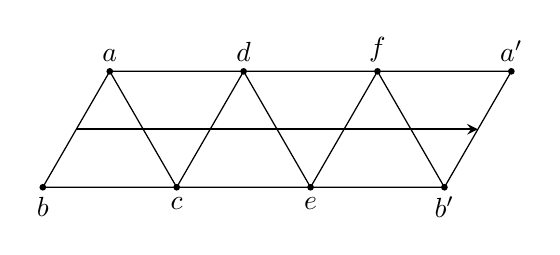
\begin{tikzpicture}[x=1.7cm,y=1.7cm,line width=.45pt,>=stealth]
\coordinate (a) at (0,.8660254); \coordinate (b) at (-.5,0);
\coordinate (c) at (.5,0); \coordinate (d) at (1,.8660254);
\coordinate (e) at (1.5,0); \coordinate (f) at (2,.8660254);
\coordinate (bp) at (2.5,0); \coordinate (ap) at (3,.8660254);
\draw (b)--(a)--(d)--(f)--(ap)--(bp)--(e)--(c)--cycle;
\draw (a)--(c)--(d)--(e)--(f)--(bp);
\draw[->,line width=.7pt] (-.25,.4330127)--(2.75,.4330127);
\foreach \p/\lab in {a/a,b/b,c/c,d/d,e/e,f/f,bp/b',ap/a'}{\fill (\p) circle (.025);}
\node[above] at (a) {$a$}; \node[above] at (d) {$d$}; \node[above] at (f) {$f$}; \node[above] at (ap) {$a'$};
\node[below] at (b) {$b$}; \node[below] at (c) {$c$}; \node[below] at (e) {$e$}; \node[below] at (bp) {$b'$};
\end{tikzpicture}
\end{center}
展开后的路线是一条直线, 每次穿越共边都按相同速度和相同角度继续, 且不经过顶点. 最后一条边与第一条边的识别在图中是平移$(3,0)$, 所以终点和出发点相同, 切向方向也相同, 可周期延续. 若八面体边长为$1$, 一周期长为$6\cdot(1/2)=3$.
\end{solution}

\begin{exercise}\label{cq:40.2}
\textbf{官方题40.2.} 平移曲面能有正的欧拉示性数吗?
\end{exercise}
\begin{solution}
不能. 第40讲中, 原三角形的一个角为$\pi a/b$, $a,b$互素正整数时, 每个对应商顶点由$2b$份该角围成, 总角为$2\pi a$, 角亏为$2\pi(1-a)\le0$. 所有顶点角亏均非正, 由定理\ref{thm:discrete-gauss-bonnet}有$2\pi\chi=\sum_v\kappa_v\le0$.

更一般的平移粘合模型也有整倍$2\pi$的锥角, 结论相同. 第40讲允许平移曲面的记账出现相同端点间的不同边, 并将边另行编号; 此时$3F=2E$及角亏计数仍成立, 所以不影响上述证明. 如需严格单纯复形, 可细分后使用同一欧拉数.
\end{solution}

\begin{exercise}\label{cq:40.3}
\textbf{官方题40.3.} 一个三角形的角为$(\pi/7,2\pi/7,4\pi/7)$. 它对应的平移曲面由多少个三角形组成? 欧拉示性数是多少?
\end{exercise}
\begin{solution}
共14个三角形, $\chi=-4$. 两条交于$\pi/7$角的边的反射复合生成$2\pi/7$旋转, 共有7种旋转. 另外两角产生的旋转已在其中, 再加上7种反射后的方向, 一共14种标记三角形的方向. 不能把仅经旋转或反射重合的三角形当成平移副本删除.

每个角的既约分母都是$7$, 对应一个商顶点需要14份该角, 而各类型角恰各有14份. 不同类型的角在边粘合时不会互相识别, 因而共有3个顶点. 闭曲面每条边邻接两面, $E=3F/2=21$, 得$\chi=3-21+14=-4$. 也可用三个顶点的角亏$0,-2\pi,-6\pi$核对: 总和为$-8\pi=2\pi\chi$.
\end{solution}
